% Build: latexmk -xelatex -interaction=nonstopmode main.tex
\documentclass[11pt,a4paper]{article}
\usepackage[margin=23mm,headheight=15pt]{geometry}
\usepackage[scheme=plain,fontset=fandol]{ctex}
\usepackage{fontspec}
\setmainfont{texgyrepagella}[Extension=.otf,UprightFont=*-regular,
 BoldFont=*-bold,ItalicFont=*-italic,BoldItalicFont=*-bolditalic]
\usepackage{amsmath,amssymb,booktabs,tabularx,longtable,array}
\usepackage{tikz}
\usetikzlibrary{arrows.meta,positioning,calc}
\usepackage{enumitem,fancyhdr,xcolor,hyperref,needspace}
\definecolor{navy}{HTML}{17334D}
\definecolor{teal}{HTML}{007E87}
\definecolor{amber}{HTML}{BA7216}
\hypersetup{colorlinks=true,linkcolor=navy,urlcolor=teal,citecolor=teal,pdftitle={Double Figure-Eight Closed-Loop Intersection Control / 双八字双路口闭环控制}}
\setlength{\parindent}{0pt}
\setlength{\parskip}{5pt}
\setlist{nosep,leftmargin=*}
\setlength{\emergencystretch}{3em}
\newcolumntype{Y}{>{\raggedright\arraybackslash}X}
\newcolumntype{P}[1]{>{\raggedright\arraybackslash}p{#1}}
\newif\ifChinese
\newcommand{\bi}[2]{\ifChinese#2\else#1\fi}
\renewcommand{\contentsname}{Contents / 目录}
\renewcommand{\figurename}{\bi{Figure}{图}}
\renewcommand{\tablename}{\bi{Table}{表}}
\renewcommand{\partname}{\bi{Part}{部分}}
\newcommand{\bisection}[2]{\Needspace{7\baselineskip}\section{\bi{#1}{#2}}}
\newcommand{\bisubsection}[2]{\Needspace{6\baselineskip}\subsection{\bi{#1}{#2}}}
\newcommand{\status}[2]{\begin{quote}\color{navy}\small\bi{#1}{#2}\end{quote}}
\pagestyle{fancy}
\fancyhf{}
\fancyhead[L]{\small\bi{Double figure-eight research design}{双八字双路口研究设计}}
\fancyhead[R]{\small\bi{Proposal / not experimental results}{研究方案 / 非实验结果}}
\fancyfoot[C]{\thepage}
\begin{document}
\hypersetup{pageanchor=false}
\begin{titlepage}
\vspace*{24mm}
{\color{teal}\large RESEARCH DESIGN \quad 研究设计\par}
\vspace{10mm}
{\color{navy}\Huge\bfseries From One Figure-Eight to\par Two Coupled Intersections\par}
\vspace{10mm}
{\LARGE\bfseries 从单八字闭环到双路口耦合\par}
\vspace{8mm}
{\large Distance-barrier control, scenario layout and experimental configuration\par}
{\large 距离 barrier 控制、场景布局与实验配置\par}
\vfill
Based on Martijn Westerhof's BSc report, student ID s5148146.\par
基于 Martijn Westerhof 的本科报告整理；完整英文版在前，完整中文版在后。\par
\vspace{5mm}
\textbf{Status / 状态：} Document and experiment design only. No new CARLA experiments or safety proof.\par
本文件为研究设计，不包含新增 CARLA 实验或已完成的安全证明。\par
\vspace{5mm}
Prepared / 整理日期：2026-10-07
\end{titlepage}
\hypersetup{pageanchor=true}
\tableofcontents
\clearpage
\Chinesefalse
\part{Complete English Version}
\bisection{Abstract and research objective}{摘要与研究目标}
\bi{The reference BSc report evaluates distance-barrier control against a fully actuated signal controller (FAS) on a single-intersection figure-eight track in CARLA. It reports better throughput, delay and energy performance for barrier control, but also transient safety violations at high density. This proposal retains the distance-based speed correction and extends the road to one closed route with two planar intersections. The central question is whether a locally formed platoon remains compatible with a second conflict point after repeated circulation.}{参考本科报告在 CARLA 的单路口八字形轨道上，对比距离 barrier 控制和全感应式信号控制（FAS）。报告中 barrier 在吞吐量、延误与能耗方面表现更好，但高密度启动阶段仍有安全违规。本方案保留基于距离的速度修正，将道路拓展为包含两个平面交叉口的一条闭合路线。核心问题是：一个路口形成的局部车队结构，在持续循环后能否同时适应另一个路口的冲突要求。}

\bi{The proposed contribution is a controlled study of inter-junction coupling, phase compatibility and transient behavior, rather than a claim of a new safety theorem. The document specifies geometry, event indexing, feedback updates, configuration and matched experiments. All new parameters are design defaults; no new simulation outcomes are presented.}{拟研究的贡献是分析路口间耦合、车队相位兼容性与瞬态行为，而不是宣称建立了新的安全定理。本文明确道路几何、事件索引、反馈更新、参数配置和配对实验。新增参数均为设计初值，文中不展示未经实施的新仿真结果。}

\status{Three evidence levels are kept separate: reported BSc observations, derived geometric facts, and proposed experimental hypotheses. ``Closed loop'' means both a closed road and repeated state feedback, not online parameter learning.}{本文区分三类证据：本科报告中的已有观察、可推导的几何事实、拟检验的实验假设。“闭环”同时指道路闭合与状态反馈更新，不指在线参数学习。}

\bisection{Reference report: outline and method}{参考报告：大纲与方法}
\bisubsection{How the original report is organized}{原报告的组织方式}
\begin{tabularx}{\linewidth}{P{.26\linewidth}Y}
\toprule
\bi{Original section}{原章节} & \bi{Role in the argument}{论证中的作用}\\
\midrule
\bi{Abstract; Introduction}{摘要；引言} & \bi{Motivation, autonomous intersection management and the comparison question.}{提出自动驾驶路口管理问题及控制方法对比目标。}\\
\bi{System Overview; Methodology}{系统概述；方法} & \bi{CARLA map, initialization, vehicle dynamics, controllers, energy model, experimental design and KPI definitions.}{介绍 CARLA 地图、初始化、车辆动力学、控制器、能耗模型、实验设计与指标。}\\
\bi{Results}{结果} & \bi{Validation, individual trajectories, barrier activations and aggregate comparison.}{展示验证、单车轨迹、barrier 激活行为及总体对比。}\\
\bi{Discussion; Conclusion}{讨论；结论} & \bi{Platoon explanation, transient safety limitations and future extensions.}{解释车队形成机制、瞬态安全局限与后续拓展。}\\
\bi{References; Appendix}{参考文献；附录} & \bi{Sources, disclosure and configuration table.}{文献来源、说明与参数配置表。}\\
\bottomrule
\end{tabularx}

\bi{The original main file includes Introduction, System Overview, Methodology, Results, Discussion and Conclusion. FigureEight and Barrier Control are methodological source components, not separate top-level chapters. A standalone file named EV Energy USage is effectively empty; the energy model is actually in Methodology. The new report should organize substantive content rather than copy the directory listing.}{原主文件依次载入引言、系统概述、方法、结果、讨论与结论。FigureEight 和 Barrier Control 是方法章节中的源文件组件，不是独立顶层章节。名为 EV Energy USage 的文件基本为空，实际能耗模型位于 Methodology。因此，新报告应按内容组织，而不是照抄文件夹中的文件名。}

\bisubsection{Single-intersection model}{单路口模型}
\bi{The reference path is}{参考路径为}
\[
 x(t)=-R\sin t,\qquad y(t)=-R\sin(2t),\qquad t\in[0,2\pi).
\]
\bi{The physical intersection has two route occurrences, at $t=0$ and $t=\pi$. Parametric position is converted to longitudinal arc length using 100,000 samples and interpolation. Vehicles are placed around the route with target spacing $L/N$ and randomized offsets; the intersection is excluded from spawning. The fleet contains Tesla Model 3 and Audi e-tron models, with one extra Tesla for odd $N$.}{同一物理交叉口在路径上出现两次，对应 $t=0$ 与 $t=\pi$。报告通过 100,000 个采样点及插值，将参数位置转换为纵向弧长。车辆按目标间距 $L/N$ 沿道路初始化，并加入随机位置扰动；交叉口内不生成车辆。车型为 Tesla Model 3 与 Audi e-tron，车辆总数为奇数时 Tesla 多一辆。}

\bi{The headway controller uses an EMA-filtered spatial gap error and a PD speed correction. A longitudinal PID converts speed error into throttle/brake, while look-ahead lateral control follows the route. For two approaching candidates, distances to their respective route occurrences of the crossing are $d_1,d_2$. The report gives}{跟驰层使用 EMA 滤波后的空间车间距误差，通过 PD 产生速度修正；纵向 PID 将速度误差转换为油门与制动，横向前视控制跟踪路线。对于两条接近分支上的候选车，到各自路口路径位置的距离为 $d_1,d_2$。报告给出的距离 barrier 为}
\[
 \Delta d=d_1-d_2,\qquad \nabla=-\frac{1}{\Delta d},\qquad
 u_{b,1}=-\frac{K_b}{\Delta d},\quad u_{b,2}=+\frac{K_b}{\Delta d}.
\]
\bi{Corrections activate when both candidates are in the approach window and $|\Delta d|$ is below the activation distance. The nearer candidate accelerates and the farther candidate decelerates. This separates distances, not explicitly predicted arrival times: equal distances with different speeds need not mean equal arrival times. The report does not provide an implementation resolving the singularity at zero.}{两辆候选车均位于接近窗口内，且 $|\Delta d|$ 小于激活距离时，修正项激活：较近的车辆加速，较远的车辆减速。这种方法分离的是距离，不是显式预测的到达时间；同距异速并不意味着同时到达。报告没有提供处理零距离差奇异点的实现代码。}

\bi{If the correction is expressed in km/h and distance in metres, $K_b$ must carry units of $(\mathrm{km/h})\,\mathrm{m}$. The original prose labels some gains and even a speed with inconsistent units. Preserve reported numerical settings but correct dimensional notation in this document; do not infer the actual code's internal units.}{若修正项以 km/h 表示、距离以 m 表示，则 $K_b$ 的量纲应为 $(\mathrm{km/h})\,\mathrm{m}$。原文部分增益及一处速度的单位标注不一致。本文保留原文数值，修正量纲表达，但不推断未取得的代码内部如何换算单位。}

\bi{FAS alternates the two conflict branches, extends green according to detection and gap-out rules, and uses the same vehicle dynamics. Battery energy integrates a mechanical force/power model and approximate motor-efficiency maps. These models are useful comparison tools, but shared approximations do not guarantee that relative energy errors cancel.}{FAS 在两条冲突分支间交替放行，根据检测与车流间隔延长绿灯，并使用相同车辆动力学。电池能耗由机械力和功率模型及近似电机效率图积分得到。这些模型可以用于比较，但两组使用相同近似，并不能保证相对能耗误差一定抵消。}

\bisection{Reported findings and limits}{已有结果与适用边界}
\begin{tabularx}{\linewidth}{P{.25\linewidth}Y}
\toprule
\bi{Metric}{指标} & \bi{Original report's observations; not new results}{原报告观察；非本研究新增结果}\\
\midrule
\bi{Throughput}{吞吐量} & \bi{Barrier approximately 0.36--0.57 veh/s across $N=51$--81; FAS approximately 0.32 veh/s at the higher densities.}{barrier 在 $N=51$--81 下约为 0.36--0.57 veh/s；FAS 在较高密度下约为 0.32 veh/s。}\\
\bi{Energy}{能耗} & \bi{Reported reductions of 20.12\%, 22.85\%, 39.97\% and 44.81\% for $N=51,61,71,81$.}{在 $N=51,61,71,81$ 下分别报告降低 20.12\%、22.85\%、39.97\% 与 44.81\%。}\\
\bi{Delay}{延误} & \bi{Reported maximum reduction of 98.86\% at $N=81$, using cumulative lap-delay accounting.}{按累计绕圈延误统计，$N=81$ 时报告最大降低 98.86\%。}\\
\bi{Safety violations}{安全违规} & \bi{Reported mean violations per run: 1.9 at $N=71$ and 21.13 at $N=81$; absent after the reported steady platoon forms.}{每次运行平均违规数：$N=71$ 时为 1.9，$N=81$ 时为 21.13；报告观察到稳态车队形成后不再新增违规。}\\
\bottomrule
\end{tabularx}

\bi{All values above come from the BSc Results and Discussion \cite{baip}; raw run data and controller scripts were not found in the supplied report directory. A lack of violations after convergence is an empirical observation, not evidence of safety from every initial condition. The 5 m violation criterion is also not identical to a geometric collision. Perfect state estimation, one crossing, no turning choices and simplified energy modeling limit transfer to a larger network.}{上表数值来自本科报告的 Results 与 Discussion\cite{baip}；所提供报告目录中未发现原始逐次实验数据或控制脚本。收敛后未观察到违规，是经验观察，不能证明任意初态下安全。原报告的 5 m 违规判据也不等同于车辆几何碰撞。理想状态估计、单交叉口、无转向选择及简化能耗模型均限制了结论向更大路网推广。}

\bi{The report cites Soltani et al. for communication-free intersection management. The verified article describes a dynamic resource acquisition graph, priority function and adaptive tolerance \cite{soltani}. It supports related-work context but does not establish that the report's inverse-distance correction is a formally proven instance of that algorithm.}{报告引用 Soltani 等的无通信路口管理工作。核实到的论文描述的是动态资源获取图、优先级函数与自适应容差\cite{soltani}。它可以用于相关工作背景，但不能据此认定本科报告的倒数距离修正是该算法的已证明实例。}

\bisection{Double figure-eight geometry and layout}{双八字道路几何与布局}
\bisubsection{One closed route, exactly two intersections}{一条闭合路线、恰好两个路口}
\bi{Use a three-lobed planar curve as a precise realization of the requested double figure-eight twist:}{采用三瓣平面曲线，将“双八字再拧一次”的想法具体化：}
\[
 x(\theta)=R\cos\theta,\qquad y(\theta)=H\sin(3\theta),\qquad R,H>0.
\]
\bi{Because equal $x$ coordinates imply equal parameters or the pair $\theta,2\pi-\theta$, distinct points coincide only when $\sin(3\theta)=0$. Excluding the ordinary closure, the two crossings are $J_1=(-R/2,0)$ and $J_2=(R/2,0)$. The path is regular everywhere: the two components of its tangent never vanish simultaneously.}{相同 $x$ 坐标要求参数相同，或形成 $\theta,2\pi-\theta$ 配对。因此，不同路径位置重合仅发生于 $\sin(3\theta)=0$。排除正常首尾闭合后，恰有两个交叉点：$J_1=(-R/2,0)$ 和 $J_2=(R/2,0)$。曲线处处正则，切向量的两个分量不会同时为零。}

\begin{figure}[htbp]
\centering
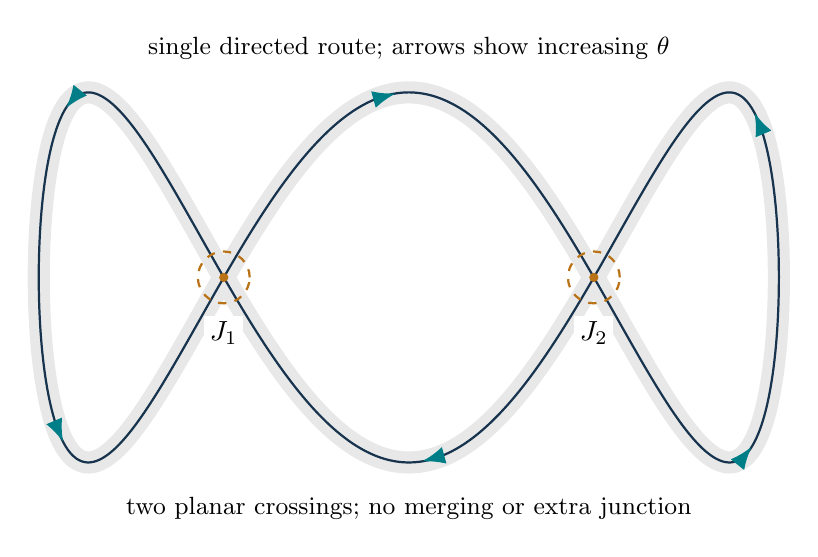
\begin{tikzpicture}[x=2.35cm,y=2.35cm,>=Latex]
 \draw[gray!18,line width=8pt,samples=501,domain=0:360,smooth,variable=\t] plot ({2*cos(\t)},{sin(3*\t)});
 \draw[navy,line width=.8pt,samples=501,domain=0:360,smooth,variable=\t] plot ({2*cos(\t)},{sin(3*\t)});
 \foreach \a in {18,85,155,198,265,335}{
  \draw[teal,very thick,->] ({2*cos(\a)},{sin(3*\a)}) -- ({2*cos(\a+3)},{sin(3*(\a+3))});}
 \foreach \x/\n in {-1/1,1/2}{
  \draw[amber,dashed,thick] (\x,0) circle (.14);
  \fill[amber] (\x,0) circle (.025);
  \node[fill=white,inner sep=2pt] at (\x,-.30) {$J_{\n}$};}
 \node[font=\small,fill=white] at (0,1.24) {\bi{single directed route; arrows show increasing $\theta$}{单条有向路线；箭头表示 $\theta$ 递增}};
 \node[font=\small,fill=white] at (0,-1.25) {\bi{two planar crossings; no merging or extra junction}{两个平面交叉点；无合流或额外路口}};
\end{tikzpicture}
\caption{\bi{Double figure-eight layout ($R/H=2$). Road width and dashed conflict regions are schematic, not to scale.}{双八字布局（$R/H=2$）。道路宽度与虚线冲突区域均为示意，不按比例绘制。}}
\end{figure}

\bi{The schematic has three enclosed lobes; it is not two independent original figure-eights joined by a merge. It expresses the agreed one-route, two-crossing topology. A physical crossing shares road space, but route branches remain fixed: vehicles cannot turn onto another branch. Build in RoadRunner as two fixed crossing junctions with branch-preserving connections and external longitudinal control.}{示意图具有三个封闭瓣区，并非通过合流连接的两个独立原八字。它实现的是已确定的“一条路线、两个交叉口”拓扑。物理路口共享道路空间，但路线分支固定，车辆不能转到其他分支。RoadRunner 中应构建两个固定交叉路口，保持分支连接，纵向控制由外部控制器负责。}

\bisubsection{Scale, curvature and event coordinates}{尺度、曲率与事件位置}
\[
 s(\theta)=\int_0^\theta\sqrt{R^2\sin^2\xi+9H^2\cos^2(3\xi)}\,d\xi,
 \qquad L=s(2\pi).
\]
\bi{For $R/H=2$ and $L=4694.8$ m, numerical integration gives $R\approx613.70$ m and $H\approx306.85$ m. The minimum centerline radius is approximately 32.31 m. At 30 km/h, the corresponding kinematic lateral acceleration is approximately 2.15 m/s$^2$; vehicle tracking must still be calibrated. The lane width is a proposed 4 m. These are new design values, not original-report parameters.}{在 $R/H=2$、$L=4694.8$ m 下，数值积分得到 $R\approx613.70$ m、$H\approx306.85$ m。中心线最小曲率半径约为 32.31 m。在 30 km/h 下，对应运动学横向加速度约为 2.15 m/s$^2$，仍需校准车辆路径跟踪。建议车道宽为 4 m。以上均为新增设计值，不是原报告配置。}

\begin{center}
\begin{tabular}{llll}
\toprule
\bi{Event}{事件} & \bi{Parameter}{参数} & \bi{Junction / branch}{路口 / 分支} & $s$ (m)\\
\midrule
$e_1$ & $\pi/3$ & $J_2/A$ & 722.67\\
$e_2$ & $2\pi/3$ & $J_1/A$ & 1624.73\\
$e_3$ & $4\pi/3$ & $J_1/B$ & 3070.07\\
$e_4$ & $5\pi/3$ & $J_2/B$ & 3972.13\\
\bottomrule
\end{tabular}
\end{center}

\begin{figure}[htbp]
\centering
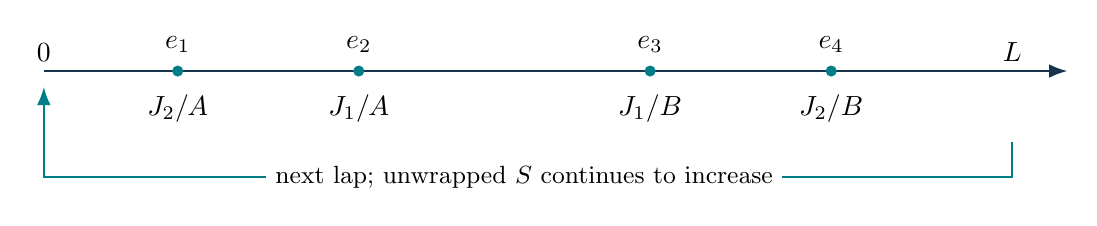
\begin{tikzpicture}[>=Latex]
 \draw[navy,thick,->] (0,0)--(13,0);
 \foreach \x/\e/\j in {1.7/1/{J_2/A},4.0/2/{J_1/A},7.7/3/{J_1/B},10.0/4/{J_2/B}}{
  \fill[teal] (\x,0) circle (2pt);
  \node[above=3pt] at (\x,0) {$e_{\e}$};
  \node[below=5pt] at (\x,0) {$\j$};}
 \node[above] at (0,0) {$0$};\node[above] at (12.3,0) {$L$};
 \draw[teal,thick,->] (12.3,-.9)--(12.3,-1.35)--(0,-1.35)--(0,-.2);
 \node[fill=white,font=\small] at (6.1,-1.35) {\bi{next lap; unwrapped $S$ continues to increase}{下一圈；展开弧长 $S$ 持续增加}};
\end{tikzpicture}
\caption{\bi{Route event order, not a physical map. Each lap has four crossing events.}{路径事件顺序，不是物理地图。每圈有四次路口通行事件。}}
\end{figure}

\bi{Consecutive event distances are approximately 902.06, 1445.34, 902.06 and 1445.34 m, including wraparound. A geometric junction separation of 613.70 m must not replace these longitudinal distances. At nominal speed, the corresponding travel times are approximately 108.25 and 173.44 s. Event order is $J_2,J_1,J_1,J_2$, not strict alternation.}{包含跨圈段在内，相邻事件的路径距离约为 902.06、1445.34、902.06 与 1445.34 m。两个路口的几何直线距离为 613.70 m，不能替代纵向路径距离。按目标速度，对应行驶时间约为 108.25 与 173.44 s。事件顺序是 $J_2,J_1,J_1,J_2$，并非严格交替。}

\bi{For every branch, obtain conflict-region entry and exit from the overlapping lane footprints, vehicle dimensions and an explicit margin. Keep these separately from the center-crossing distance used by the barrier. Do not draw a circular region and then assume it defines a validated safety threshold.}{各分支的冲突区域入口与出口，应根据车道占地重叠、车辆尺寸及明确余量确定。它们与 barrier 使用的中心交叉断面距离分别记录。不能仅画一个圆形示意区域，就将其视为经过验证的安全阈值。}

\bisection{Feedback control at two junctions}{两个路口的反馈控制}
\bisubsection{State and event interfaces}{状态与事件接口}
\bi{Use wrapped position $s_i\in[0,L)$ and unwrapped position $S_i=s_i+n_iL$. Each encounter has an event ID, junction ID, branch ID and lap index. Track route progress using the previous branch and a local projection window; nearest Euclidean point alone is ambiguous at a crossing. Center-crossing distance is the signed difference between the encounter coordinate and $S_i$.}{使用圈内位置 $s_i\in[0,L)$ 与展开位置 $S_i=s_i+n_iL$。每次路口经过均包含事件 ID、路口 ID、分支 ID 和圈数。根据上一时刻分支与局部投影窗口跟踪路径进度；仅使用最近欧氏点会在路口产生歧义。到交叉中心断面的距离为该次事件位置与 $S_i$ 的有符号差。}

\begin{tabularx}{\linewidth}{P{.23\linewidth}Y}
\toprule
\bi{Module}{模块} & \bi{Minimum interface}{最小接口}\\
\midrule
\bi{State mapping}{状态映射} & \bi{Vehicle ID, timestamp, $S_i$, $v_i$, branch/event ID, measured body dimensions.}{车辆 ID、时间戳、$S_i$、$v_i$、分支与事件 ID、实际车身尺寸。}\\
\bi{Local candidate selection}{局部候选选择} & \bi{For each junction: nearest approaching candidate per branch within $D_a$; occupied branches logged separately.}{每路口：各分支接近窗口 $D_a$ 内最近候选车；占用分支另行记录。}\\
\bi{Speed correction}{速度修正} & \bi{Two distances, gain, activation and saturation; output signed correction and activation flag.}{两个距离、增益、激活与饱和参数；输出有符号修正及激活标记。}\\
\bi{Execution and logging}{执行与记录} & \bi{Target and actual speed, throttle/brake, saturation, event crossing, rear clearance, collision and proximity records.}{目标与实际速度、油门制动、饱和、中心通行、车尾离开、碰撞及接近事件记录。}\\
\bottomrule
\end{tabularx}

\bi{The simulator may provide complete state for experiment orchestration. The barrier's decision input remains local own/conflicting-vehicle state, route geometry and a fixed branch tie rule; it does not use downstream queues or a central schedule. Ideal availability of local measurements is assumed first. This is not a demonstrated onboard perception system.}{仿真器可为实验组织提供完整状态，但 barrier 决策仅使用局部本车与冲突车状态、路线几何和固定分支平局规则，不使用下游队列或集中调度。首轮先假设局部测量理想可用；这不等同于已经实现车载感知系统。}

\bisubsection{An explicit engineering variant}{明确区分的工程改写版本}
\bi{Because original code is unavailable, label the following as a regularized distance-barrier baseline, not exact reproduction. Set $\varepsilon=0.1$ m as a numerical design default. If $|\Delta d|\ge\varepsilon$, use $\widehat{\Delta d}=\Delta d$. Otherwise set its magnitude to $\varepsilon$ with the observed sign; at exact equality, assign branch A to pass first, hence $\widehat{\Delta d}=-\varepsilon$.}{由于未获得原代码，下式应标注为“正则化距离 barrier 基线”，而非精确复现。取 $\varepsilon=0.1$ m 作为数值设计初值。当 $|\Delta d|\ge\varepsilon$ 时，取 $\widehat{\Delta d}=\Delta d$；否则将绝对值设为 $\varepsilon$，保留观测符号。严格相等时，固定 A 分支先行，因此取 $\widehat{\Delta d}=-\varepsilon$。}
\[
 u_{b,1}=\operatorname{clip}\!\left(-K_b/\widehat{\Delta d},-7,7\right),\quad
 u_{b,2}=-u_{b,1}\quad (\mathrm{km/h}).
\]
\bi{For a non-candidate or inactive pair, $u_b=0$. Compute one command per vehicle:}{非候选车辆或未激活的冲突对取 $u_b=0$。每辆车每周期生成一个指令：}
\[
 v_i^{cmd}=\operatorname{clip}\!\left(30+u_{h,i}+u_{b,i},0,40\right)\quad(\mathrm{km/h}),
 \qquad |u_{h,i}|\le10\ \mathrm{km/h}.
\]
\bi{The 40 km/h command ceiling and additive fusion are proposed choices, not confirmed original settings. Retain the report's PD/PID numbers initially, declare gap error as actual minus target spacing, and use metres/seconds for gap derivatives. Convert explicitly when entering a km/h speed loop. EMA is defined here as filtered error $\bar e_k=0.9\bar e_{k-1}+0.1e_k$; the original alpha convention is unknown.}{40 km/h 指令上限与加法融合是建议选择，不是已确认的原配置。首轮保留报告中的 PD/PID 数值，约定间距误差为实际间距减目标间距，间距导数使用 m 与 s；进入 km/h 速度环时显式换算。本文 EMA 定义为 $\bar e_k=0.9\bar e_{k-1}+0.1e_k$，原代码的 alpha 约定仍未知。}

\bi{Do not claim that a nominal barrier gain ``dominates'' headway control: saturation and opposite corrections may cancel it. Log the two components before fusion and the final clipped speed. The tie rule, reciprocal regularization and nearest-candidate reduction are heuristics, not collision-avoidance proofs. Downstream occupants remain in the occupancy ledger until their rear clears, but that ledger alone does not change the distance law or guarantee safe release.}{不能仅因增益较大，就宣称 barrier “主导”跟驰控制：饱和及相反修正仍可能抵消其作用。应记录融合前的两个分量和最终限幅速度。平局规则、倒数正则化及最近候选车筛选均为启发式处理，不是避碰证明。下游占用车辆保留至车尾离开，但占用记录本身不会改变距离控制律，也不保证安全放行。}

\bisubsection{Update order and propagation mechanism}{更新顺序与扰动传播}
\begin{figure}[htbp]
\centering
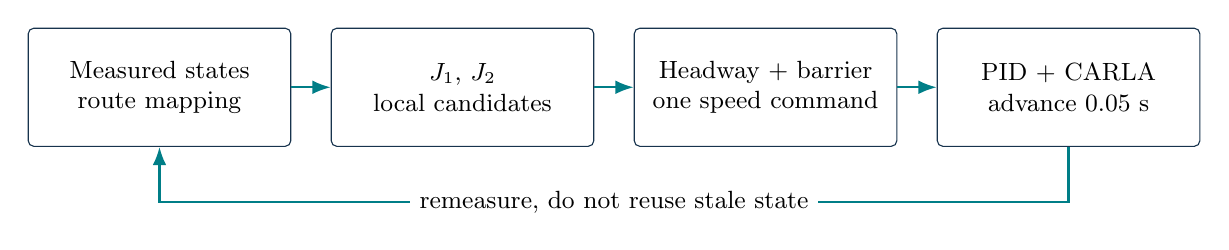
\begin{tikzpicture}[>=Latex,node distance=5mm,
 box/.style={draw=navy,rounded corners=2pt,align=center,font=\small,text width=31mm,minimum height=15mm},
 arr/.style={->,thick,teal}]
 \node[box] (state) {\bi{Measured states\\route mapping}{实际状态\\路径映射}};
 \node[box,right=of state] (local) {\bi{$J_1$, $J_2$\\local candidates}{ $J_1$、$J_2$\\局部候选车}};
 \node[box,right=of local] (speed) {\bi{Headway + barrier\\one speed command}{跟驰 + barrier\\单一速度指令}};
 \node[box,right=of speed] (plant) {\bi{PID + CARLA\\advance 0.05 s}{PID + CARLA\\推进 0.05 s}};
 \draw[arr] (state)--(local);\draw[arr] (local)--(speed);\draw[arr] (speed)--(plant);
 \draw[arr] (plant.south)--++(0,-.7)-|(state.south);
 \node[font=\small,fill=white] at ($(local.south)!0.5!(speed.south)+(0,-.7)$) {\bi{remeasure, do not reuse stale state}{重新测量，不沿用旧状态}};
\end{tikzpicture}
\caption{\bi{Synchronous state feedback; junction computations use the same snapshot.}{同步状态反馈；两个路口使用同一时刻的状态快照。}}
\end{figure}

\begin{enumerate}
\item \bi{Read one snapshot; update unwrapped progress, predecessor gaps and encounter/occupancy records.}{读取一次状态快照，更新展开位置、前车间距以及事件与占用记录。}
\item \bi{Select local candidates independently at both junctions from that snapshot.}{依据同一快照，分别选择两个路口的局部候选车。}
\item \bi{Compute headway and local barrier corrections, fuse once and execute throttle/brake commands.}{计算跟驰与局部 barrier 修正，统一融合一次后执行油门制动指令。}
\item \bi{Advance the physics by one step; detect crossing and rear-clearance transitions without resetting the same encounter prematurely.}{推进一个物理步长；检测通行与车尾离开，避免过早重置同一次路口经过事件。}
\item \bi{Record actual response and safety events, then repeat using newly measured states.}{记录实际响应及安全事件，随后使用新测量状态重复更新。}
\end{enumerate}

\bi{With 20--60 m windows, consecutive events are separated by much more than twice the window length in the proposed geometry. A vehicle therefore receives at most one local barrier correction at a time. Long-range effects arise through changed travel times and predecessor gaps, not simultaneous summation of junction commands. Any enlarged-window case that violates this separation is outside the present baseline.}{在所提几何中，20--60 m 窗口远小于相邻事件距离的一半，因此每辆车同一时刻最多接受一个局部 barrier 修正。跨路口影响通过行驶时间及前后车间距变化传播，不来自两个路口指令的同时求和。若进一步扩大窗口破坏该条件，则超出本基线适用范围。}

\bi{A correction at $J_1$ changes speed and spacing before a later $J_2$ encounter; repeated circulation returns those changes to $J_1$. Consecutive visits to the same junction also matter. Hypotheses are: compatible phases permit low-intervention circulation; incompatible phases cause recurring interventions; higher density or asymmetric path lengths amplify the coupling. All three must be tested, not asserted.}{$J_1$ 的修正改变车辆速度与间距，影响后续 $J_2$ 的到达；持续循环后，这些变化又返回 $J_1$。连续两次经过同一路口也会影响反馈。待检验假设是：相位兼容时可形成低干预循环；相位不兼容时会反复激活；更高密度或不对称路径长度可能放大耦合。这些均须实验验证。}

\Needspace{16\baselineskip}
\bisection{Configuration and matched experiments}{配置与配对实验}
\bisubsection{Parameter register}{参数登记表}
\begin{longtable}{P{.34\linewidth}P{.33\linewidth}P{.23\linewidth}}
\toprule
\bi{Parameter}{参数} & \bi{Value}{取值} & \bi{Status}{状态}\\
\midrule\endhead
\bi{Reference track length}{原轨道长度} & 2347.4 m & \bi{BSc report}{本科报告}\\
\bi{Double track length; width}{双路口长度；车道宽} & 4694.8 m; 4 m & \bi{Proposed}{建议}\\
$R/H$ & 2; \bi{diagnostics: 1.5, 3}{诊断值：1.5、3} & \bi{Proposed}{建议}\\
\bi{Target speed; timestep}{目标速度；步长} & 30 km/h; 0.05 s & \bi{BSc report}{本科报告}\\
\bi{Duration; preparation; ramp}{时长；准备；加速} & 1800 s; 5 s; 12.5 s & \bi{BSc report}{本科报告}\\
\bi{Single-junction counts}{单路口车辆数} & 51, 61, 71, 81 & \bi{BSc report}{本科报告}\\
\bi{Double-junction counts}{双路口车辆数} & 102, 122, 142, 162 & \bi{Density matched}{匹配密度}\\
\bi{Spawn noise; repetitions}{初始化扰动；重复次数} & $\pm20\%$; 30 & \bi{BSc report}{本科报告}\\
$K_b$; $D_{activation}$; $D_a$ & 25; 10 m; 20 m & \bi{Appendix B}{原附录 B}\\
\bi{Barrier correction limit}{barrier 修正上限} & $\pm7$ km/h & \bi{BSc Discussion}{原讨论章节}\\
\bi{Headway PD; EMA}{跟驰 PD；EMA} & 3.5, 1.0; 0.9 & \bi{Numbers from Appendix}{数值来自原附录}\\
\bi{Longitudinal PID}{纵向 PID} & 0.5, 0.25, 0.02 & \bi{Numbers from Appendix}{数值来自原附录}\\
\bi{Regularization; speed ceiling}{正则化；指令速度上限} & 0.1 m; 40 km/h & \bi{Engineering variant}{工程改写}\\
\bi{Command units, EMA convention}{指令单位、EMA 约定} & \bi{Explicit variant definitions}{采用改写版本的明确约定} & \bi{Original code unknown}{原代码未知}\\
\bottomrule
\end{longtable}

\bi{FAS defaults from the original Appendix B are: stop line 12 m upstream, approach window 50 m, reaction time 1 s, assumed deceleration 2.5 m/s$^2$, minimum/maximum green 12/45 s, yellow 4 s, gap-out 3.4 s, upstream detector offset 30 m, request loop length 10 m and discharge loop length 5 m. Appendix B also lists a ``maximum yellow time'' of 1 s, inconsistent with yellow 4 s. Use 4 s in the declared engineering baseline and retain the 1 s entry as an unresolved source discrepancy. Apply the same independent FAS to each junction; no green-wave offsets.}{原附录 B 中 FAS 参数为：停止线在路口上游 12 m、接近窗口 50 m、反应时间 1 s、假设减速度 2.5 m/s$^2$、最小/最大绿灯 12/45 s、黄灯 4 s、间隔终止阈值 3.4 s、上游检测器偏移 30 m、请求线圈长 10 m、放行线圈长 5 m。附录还列出“最大黄灯时间”1 s，与黄灯 4 s 不一致。声明的工程基线采用 4 s，并保留 1 s 项作为待核实的来源矛盾。两个路口分别运行同一 FAS，不加入绿波偏移。}

\bi{Freeze the installed CARLA/RoadRunner versions, map export settings, vehicle blueprints and physics parameters after a smoke test. The original report does not identify a CARLA version. Keep throttle/brake mutually exclusive and avoid velocity overrides after initialization. Record simulator collision protection, intervention, removal and respawn behavior rather than attributing it to the controller.}{在试运行后冻结实际安装的 CARLA/RoadRunner 版本、地图导出设置、车辆蓝图和物理参数。原报告未明确 CARLA 版本。油门与制动互斥，初始化后不直接覆盖车辆速度。记录仿真器的碰撞保护、干预、移除及重新生成行为，不能将这些机制计入控制器自身能力。}

\bisubsection{Experiment stages and controls}{实验阶段与对照}
\begin{enumerate}
\item \bi{Reference check: rebuild the original single-junction geometry and run the regularized barrier and FAS at the four original counts. Compare qualitative trajectories; exact numeric reproduction remains unclaimed without original code.}{参考检查：重建原单路口几何，在四组原车辆数下运行正则化 barrier 与 FAS。比较定性轨迹；缺少原代码时不宣称精确数值复现。}
\item \bi{Primary double-junction experiment: compare regularized barrier and independent FAS at the four doubled counts. Use 30 paired seeds (0--29), with identical spawn/type assignments within each comparison. Use separate tuning seeds 100--109.}{双路口主实验：在四组翻倍车辆数下，对比正则化 barrier 与独立 FAS。采用 30 个配对种子（0--29），每组控制器共享初始化与车型分配。调参种子另用 100--109。}
\item \bi{Geometry diagnostic: hold $L$, density and controller fixed; vary $R/H$ over 1.5, 2, 3. At 1.5 the minimum radius is about 20.21 m, so tracking and lateral acceleration are a confound. Calibrate before use; if the common speed is infeasible, classify it as a geometry stress case, not a clean coupling comparison.}{几何诊断：固定 $L$、密度和控制器，比较 $R/H=1.5,2,3$。比例 1.5 时最小半径约为 20.21 m，跟踪能力与横向加速度会成为混杂因素。先校准；若共同速度不可行，则归为几何压力案例，而非纯耦合对比。}
\item \bi{Control-window diagnostic: vary $D_a=20,40,60$ m at fixed geometry and density, leaving gain and activation distance unchanged. Repeat at $N-1$ and $N+1$ to examine initialization phase/parity, separately from the matched-density main experiment.}{控制窗口诊断：固定几何和密度，比较 $D_a=20,40,60$ m，保持增益与激活距离不变。另在 $N-1$ 与 $N+1$ 下检查初始化相位与奇偶性，独立于匹配密度的主实验。}
\end{enumerate}

\bi{At doubled $L$ and $N$, target center spacing $L/N$ remains the original value. Even counts use equal type numbers. Odd diagnostics use one extra Tesla. Treat spacing as center-to-center unless explicitly converting to bumper gap. Use safe spawn screening outside both conflict regions with full vehicle footprints; do not snap several vehicles to the same safe waypoint. Reject and resample an entire infeasible placement with deterministic attempt indexing, recording every rejection.}{长度与车辆数同时翻倍后，目标中心间距 $L/N$ 与原报告一致。偶数车辆使用相同数量的两种车型；奇数诊断中 Tesla 多一辆。间距默认指中心到中心距离，若转换为车身净间距必须明确。初始化时按完整车身占地排除两个冲突区域，避免将多辆车吸附到同一安全路点。对于不可行的整组位置，按确定性的尝试索引重新采样，并记录所有拒绝。}

\bi{Primary runs last 1800 s. Report initialization/ramp separately, the early transient through 600 s, and the later 600--1800 s window, without automatically calling it steady state. A declared non-convergence follow-up may extend every seed of an affected condition to 3600 s; do not extend only favorable runs.}{主实验时长为 1800 s。分别报告初始化与加速阶段、截至 600 s 的早期瞬态，以及 600--1800 s 的后期窗口，不自动将后期称为稳态。若某条件未收敛，可按事先声明的后续实验将该条件的全部种子延长至 3600 s，不能只延长有利样本。}

\bisection{Metrics, analysis and acceptance tests}{指标、分析与验收测试}
\bisubsection{Comparable network accounting}{可比较的网络统计口径}
\bi{Count passage once per vehicle/event/lap using a signed-distance transition, rather than counting frames spent near a crossing. Report each $Q_j=C_j/T$ separately, plus route lap completions $Q_{lap}$. A lap has two crossing events in the original geometry and four in the new one. Consequently the sum $Q_1+Q_2$ cannot alone demonstrate a throughput improvement over the single intersection. At uniform target speed the kinematic references are $Q_{lap}=Nv^*/L$ and total crossing rate $4Nv^*/L$ for the new path. They are nominal-speed references, not strict upper bounds when commanded speeds exceed $v^*$.}{按车辆、事件和圈数，以有符号距离跨越计数，每次通行只计一次，不能将停留在路口附近的每帧都算作通行。分别报告 $Q_j=C_j/T$ 及整圈完成率 $Q_{lap}$。原路线每圈两次通行，新路线每圈四次，因此仅凭 $Q_1+Q_2$ 不能认定相对单路口的吞吐量提升。匀速目标速度下，新路线的运动学参考值为 $Q_{lap}=Nv^*/L$ 与总通行率 $4Nv^*/L$。若指令速度允许超过 $v^*$，这些是目标速度参考值，不是严格上界。}

\bi{Delay is actual completed-lap time minus a one-vehicle free-flow lap time on the same geometry and tracking setup. Also report incomplete laps and elapsed time; clipping negative delay to zero must not be silently introduced. Energy is total battery kWh divided by actual traveled kilometres, with type-stratified results. Report collision contacts, overlapping occupancy of conflicting branches and the original-style 5 m proximity threshold separately. Because the source does not define its exact proximity implementation, use a declared new criterion: at one candidate's center crossing, count an event if the opposite approaching candidate is less than 5 m from its center crossing, deduplicated by vehicle pair and encounter. This is a proximity event, not a reproduced original collision count.}{延误为完成一圈的实际时间减去同几何、同跟踪设置下单车自由流圈时。另报告未完成圈次及已行驶时间，不能静默将负延误截断为零。能耗为总电池 kWh 除以实际行驶 km，并按车型分层。几何接触、冲突分支区域占用重叠及原风格的 5 m 接近阈值分别统计。原文未定义接近事件的准确实现，因此声明一个新判据：某候选车中心过线时，若另一冲突分支接近车到其中心断面不足 5 m，则记录一次；按车辆对与事件去重。这是接近事件，不是已复现的原碰撞计数。}

\bi{Track activation frequency, headway RMS error, minimum body clearance, speed/acceleration variability, command saturation and stops (speed below 0.1 m/s for at least 1 s). Operational convergence means all center-spacing errors stay within 2.5 m and no barrier activation occurs for at least one nominal full-lap duration. This is a measured criterion, not stability proof. Use cross-correlation or event-aligned changes in speed/gap between junctions to estimate propagation delay; distinguish association from causality.}{记录激活频率、车间距 RMS 误差、最小车身间距、速度与加速度波动、指令饱和及停车（速度低于 0.1 m/s 持续至少 1 s）。操作性收敛定义为：全部中心间距误差保持在 2.5 m 内，且至少一个目标速度完整圈时内无 barrier 激活。这是测量判据，不是稳定性证明。通过两路口速度或间距变化的互相关及事件对齐估计传播时延，并区分统计关联与因果结论。}

\bi{Compute metrics per seed first. Report means and paired method differences with seed-level bootstrap 95\% intervals (10,000 resamples, fixed analysis seed 20261007). Do not treat vehicle observations as independent experimental repetitions. Preserve all failed runs, controller interventions and uncompleted trajectories.}{先按种子计算指标，再报告均值与方法间配对差，采用种子层面的 bootstrap 95\% 区间（10,000 次重采样，分析种子固定为 20261007）。不能将同次运行内的车辆观察视为独立实验重复。保留所有运行失败、控制干预及未完成轨迹。}

\bisubsection{Required scenarios before batch experiments}{批量实验前的必查场景}
\begin{tabularx}{\linewidth}{P{.35\linewidth}Y}
\toprule
\bi{Scenario}{场景} & \bi{Acceptance observation}{验收观察}\\
\midrule
\bi{One vehicle, multiple laps}{单车连续绕圈} & \bi{Exactly four events per lap; no false pairs or progress jumps.}{每圈恰好四次事件，无虚假冲突对或路径位置跳变。}\\
\bi{Equal distance; unequal speeds}{等距离；不同速度} & \bi{Finite deterministic commands; differing behavior is logged, not declared safe.}{指令有限且确定；记录行为差异，不预先认定安全。}\\
\bi{Crossing and lap boundary}{过路口与跨圈} & \bi{Correct branch IDs, one crossing count and rear-clearance retention.}{分支 ID 正确、通行只计一次、车尾未离开时保留占用。}\\
\bi{Two followers and a crossing car}{两辆跟驰车与横向来车} & \bi{Headway/barrier cancellation, saturation and collisions remain visible.}{跟驰与 barrier 抵消、饱和及碰撞均可观察。}\\
\bi{Dense randomized initialization}{高密度随机初始化} & \bi{Safe spawning; transient violations and rejected placements reported.}{生成时无车身重叠；报告瞬态违规及位置拒绝。}\\
\bi{One-junction speed perturbation}{单路口速度扰动} & \bi{Follow perturbation through downstream visits and back around the loop.}{追踪扰动经过下游路口并绕回的过程。}\\
\bi{0.05 s versus 0.025 s replay}{0.05 s 与 0.025 s 重放} & \bi{Check sampling sensitivity and independent body/occupancy events.}{检查采样敏感性及独立车身和占用事件。}\\
\bottomrule
\end{tabularx}

\clearpage
\bisection{Implementation roadmap and decision boundary}{实施路线与决策边界}
\begin{enumerate}
\item \bi{Geometry milestone: generate the curve and arc-length table, verify exactly two crossings, four encounters, curvature and branch connections; calibrate one vehicle.}{几何阶段：生成曲线与弧长表，验证两个交叉点、四次经过、曲率及分支连接；完成单车校准。}
\item \bi{Control milestone: implement the declared regularized baseline and independent FAS, verify state/event bookkeeping, then test transient failure cases.}{控制阶段：实施声明的正则化基线与独立 FAS，验证状态和事件记录，再检查瞬态失败案例。}
\item \bi{Experiment milestone: freeze configuration and tuning, execute paired seeds, analyze efficiency together with safety and convergence.}{实验阶段：冻结配置及调参结果，运行配对种子，将效率、安全和收敛一并分析。}
\item \bi{Extension milestone: only after diagnosing the coupling, consider local adaptive gain or occupancy-aware release as separately named variants. Shared-state junction coordination and acceleration-QP filtering remain outside the present method.}{拓展阶段：诊断耦合机制后，再将局部自适应增益或占用感知放行作为独立命名的改进版本。共享状态路口协调与加速度 QP 过滤不属于当前方法。}
\end{enumerate}

\bi{A useful study may discover a failure boundary rather than improved performance. The main deliverable is an auditable relationship between geometry, density, local interventions and global circulation. If repeated interventions persist or transient safety worsens, report those outcomes and narrow the operating domain before adding more junctions.}{研究可能发现的是失效边界，而非性能提升。核心交付是可核查的几何、密度、局部干预与全局循环之间的关系。若持续反复激活或瞬态安全恶化，应如实报告，并先收缩适用范围，再增加路口数量。}

\bisection{Appendix: files, pseudocode and open items}{附录：文件、伪代码与待核实事项}
\begingroup\small
\bi{The editable package includes the main file (main.tex), bilingual body (report\_body.tex), bibliography (references.bib), design register (proposed\_config.json), geometry results (geometry\_summary.json), and checker (geometry\_check.py). The body is rendered twice with one language switch, sharing formulas and TikZ geometry. Build with \texttt{latexmk -xelatex main.tex}.}{文件包包括主文件（main.tex）、双语正文（report\_body.tex）、文献库（references.bib）、设计登记表（proposed\_config.json）、几何结果（geometry\_summary.json）与检查脚本（geometry\_check.py）。正文通过语言开关渲染两次，共用公式与 TikZ 几何。使用 \texttt{latexmk -xelatex main.tex} 编译。}

\begin{quote}\small
\bi{Initialize map, vehicles, event ledger and logs. For each synchronous tick: snapshot state; map route progress; update predecessor and occupancy records; select the two local pairs; calculate PD and active regularized corrections; fuse/clamp the speed once; execute PID throttle/brake; advance CARLA; record actual response and events. After each run: preserve failures and unfinished laps; aggregate per seed.}{初始化地图、车辆、事件台账与日志。每个同步周期：获取状态快照；映射路径进度；更新前车与占用记录；选择两个局部冲突对；计算 PD 和激活的正则化修正；统一融合并限幅速度；执行 PID 油门制动；推进 CARLA；记录实际响应和事件。每次运行结束：保留失败与未完成圈次，按种子汇总指标。}
\end{quote}

\bi{Open items before executable experiments: original controller code and signal phase details; speed-loop units and PID discretization; EMA convention; handling of rear occupancy; original proximity counter; map export/version compatibility; blueprint dimensions and per-type braking/tracking calibration. No executable API is added to the project by this document. The JSON is a design register, not a working CARLA configuration.}{运行仿真实验前，仍需核实原控制代码与信号相位细节、速度环单位及 PID 离散化、EMA 约定、车尾占用处理、原接近事件计数器、地图导出与版本兼容、车辆蓝图尺寸，以及各车型的制动和跟踪表现。本文件不新增可执行控制 API；JSON 用于登记设计参数，不能直接作为 CARLA 配置运行。}
\endgroup

\clearpage
\Chinesetrue
\part{完整中文版}
\bisection{Abstract and research objective}{摘要与研究目标}
\bi{The reference BSc report evaluates distance-barrier control against a fully actuated signal controller (FAS) on a single-intersection figure-eight track in CARLA. It reports better throughput, delay and energy performance for barrier control, but also transient safety violations at high density. This proposal retains the distance-based speed correction and extends the road to one closed route with two planar intersections. The central question is whether a locally formed platoon remains compatible with a second conflict point after repeated circulation.}{参考本科报告在 CARLA 的单路口八字形轨道上，对比距离 barrier 控制和全感应式信号控制（FAS）。报告中 barrier 在吞吐量、延误与能耗方面表现更好，但高密度启动阶段仍有安全违规。本方案保留基于距离的速度修正，将道路拓展为包含两个平面交叉口的一条闭合路线。核心问题是：一个路口形成的局部车队结构，在持续循环后能否同时适应另一个路口的冲突要求。}

\bi{The proposed contribution is a controlled study of inter-junction coupling, phase compatibility and transient behavior, rather than a claim of a new safety theorem. The document specifies geometry, event indexing, feedback updates, configuration and matched experiments. All new parameters are design defaults; no new simulation outcomes are presented.}{拟研究的贡献是分析路口间耦合、车队相位兼容性与瞬态行为，而不是宣称建立了新的安全定理。本文明确道路几何、事件索引、反馈更新、参数配置和配对实验。新增参数均为设计初值，文中不展示未经实施的新仿真结果。}

\status{Three evidence levels are kept separate: reported BSc observations, derived geometric facts, and proposed experimental hypotheses. ``Closed loop'' means both a closed road and repeated state feedback, not online parameter learning.}{本文区分三类证据：本科报告中的已有观察、可推导的几何事实、拟检验的实验假设。“闭环”同时指道路闭合与状态反馈更新，不指在线参数学习。}

\bisection{Reference report: outline and method}{参考报告：大纲与方法}
\bisubsection{How the original report is organized}{原报告的组织方式}
\begin{tabularx}{\linewidth}{P{.26\linewidth}Y}
\toprule
\bi{Original section}{原章节} & \bi{Role in the argument}{论证中的作用}\\
\midrule
\bi{Abstract; Introduction}{摘要；引言} & \bi{Motivation, autonomous intersection management and the comparison question.}{提出自动驾驶路口管理问题及控制方法对比目标。}\\
\bi{System Overview; Methodology}{系统概述；方法} & \bi{CARLA map, initialization, vehicle dynamics, controllers, energy model, experimental design and KPI definitions.}{介绍 CARLA 地图、初始化、车辆动力学、控制器、能耗模型、实验设计与指标。}\\
\bi{Results}{结果} & \bi{Validation, individual trajectories, barrier activations and aggregate comparison.}{展示验证、单车轨迹、barrier 激活行为及总体对比。}\\
\bi{Discussion; Conclusion}{讨论；结论} & \bi{Platoon explanation, transient safety limitations and future extensions.}{解释车队形成机制、瞬态安全局限与后续拓展。}\\
\bi{References; Appendix}{参考文献；附录} & \bi{Sources, disclosure and configuration table.}{文献来源、说明与参数配置表。}\\
\bottomrule
\end{tabularx}

\bi{The original main file includes Introduction, System Overview, Methodology, Results, Discussion and Conclusion. FigureEight and Barrier Control are methodological source components, not separate top-level chapters. A standalone file named EV Energy USage is effectively empty; the energy model is actually in Methodology. The new report should organize substantive content rather than copy the directory listing.}{原主文件依次载入引言、系统概述、方法、结果、讨论与结论。FigureEight 和 Barrier Control 是方法章节中的源文件组件，不是独立顶层章节。名为 EV Energy USage 的文件基本为空，实际能耗模型位于 Methodology。因此，新报告应按内容组织，而不是照抄文件夹中的文件名。}

\bisubsection{Single-intersection model}{单路口模型}
\bi{The reference path is}{参考路径为}
\[
 x(t)=-R\sin t,\qquad y(t)=-R\sin(2t),\qquad t\in[0,2\pi).
\]
\bi{The physical intersection has two route occurrences, at $t=0$ and $t=\pi$. Parametric position is converted to longitudinal arc length using 100,000 samples and interpolation. Vehicles are placed around the route with target spacing $L/N$ and randomized offsets; the intersection is excluded from spawning. The fleet contains Tesla Model 3 and Audi e-tron models, with one extra Tesla for odd $N$.}{同一物理交叉口在路径上出现两次，对应 $t=0$ 与 $t=\pi$。报告通过 100,000 个采样点及插值，将参数位置转换为纵向弧长。车辆按目标间距 $L/N$ 沿道路初始化，并加入随机位置扰动；交叉口内不生成车辆。车型为 Tesla Model 3 与 Audi e-tron，车辆总数为奇数时 Tesla 多一辆。}

\bi{The headway controller uses an EMA-filtered spatial gap error and a PD speed correction. A longitudinal PID converts speed error into throttle/brake, while look-ahead lateral control follows the route. For two approaching candidates, distances to their respective route occurrences of the crossing are $d_1,d_2$. The report gives}{跟驰层使用 EMA 滤波后的空间车间距误差，通过 PD 产生速度修正；纵向 PID 将速度误差转换为油门与制动，横向前视控制跟踪路线。对于两条接近分支上的候选车，到各自路口路径位置的距离为 $d_1,d_2$。报告给出的距离 barrier 为}
\[
 \Delta d=d_1-d_2,\qquad \nabla=-\frac{1}{\Delta d},\qquad
 u_{b,1}=-\frac{K_b}{\Delta d},\quad u_{b,2}=+\frac{K_b}{\Delta d}.
\]
\bi{Corrections activate when both candidates are in the approach window and $|\Delta d|$ is below the activation distance. The nearer candidate accelerates and the farther candidate decelerates. This separates distances, not explicitly predicted arrival times: equal distances with different speeds need not mean equal arrival times. The report does not provide an implementation resolving the singularity at zero.}{两辆候选车均位于接近窗口内，且 $|\Delta d|$ 小于激活距离时，修正项激活：较近的车辆加速，较远的车辆减速。这种方法分离的是距离，不是显式预测的到达时间；同距异速并不意味着同时到达。报告没有提供处理零距离差奇异点的实现代码。}

\bi{If the correction is expressed in km/h and distance in metres, $K_b$ must carry units of $(\mathrm{km/h})\,\mathrm{m}$. The original prose labels some gains and even a speed with inconsistent units. Preserve reported numerical settings but correct dimensional notation in this document; do not infer the actual code's internal units.}{若修正项以 km/h 表示、距离以 m 表示，则 $K_b$ 的量纲应为 $(\mathrm{km/h})\,\mathrm{m}$。原文部分增益及一处速度的单位标注不一致。本文保留原文数值，修正量纲表达，但不推断未取得的代码内部如何换算单位。}

\bi{FAS alternates the two conflict branches, extends green according to detection and gap-out rules, and uses the same vehicle dynamics. Battery energy integrates a mechanical force/power model and approximate motor-efficiency maps. These models are useful comparison tools, but shared approximations do not guarantee that relative energy errors cancel.}{FAS 在两条冲突分支间交替放行，根据检测与车流间隔延长绿灯，并使用相同车辆动力学。电池能耗由机械力和功率模型及近似电机效率图积分得到。这些模型可以用于比较，但两组使用相同近似，并不能保证相对能耗误差一定抵消。}

\bisection{Reported findings and limits}{已有结果与适用边界}
\begin{tabularx}{\linewidth}{P{.25\linewidth}Y}
\toprule
\bi{Metric}{指标} & \bi{Original report's observations; not new results}{原报告观察；非本研究新增结果}\\
\midrule
\bi{Throughput}{吞吐量} & \bi{Barrier approximately 0.36--0.57 veh/s across $N=51$--81; FAS approximately 0.32 veh/s at the higher densities.}{barrier 在 $N=51$--81 下约为 0.36--0.57 veh/s；FAS 在较高密度下约为 0.32 veh/s。}\\
\bi{Energy}{能耗} & \bi{Reported reductions of 20.12\%, 22.85\%, 39.97\% and 44.81\% for $N=51,61,71,81$.}{在 $N=51,61,71,81$ 下分别报告降低 20.12\%、22.85\%、39.97\% 与 44.81\%。}\\
\bi{Delay}{延误} & \bi{Reported maximum reduction of 98.86\% at $N=81$, using cumulative lap-delay accounting.}{按累计绕圈延误统计，$N=81$ 时报告最大降低 98.86\%。}\\
\bi{Safety violations}{安全违规} & \bi{Reported mean violations per run: 1.9 at $N=71$ and 21.13 at $N=81$; absent after the reported steady platoon forms.}{每次运行平均违规数：$N=71$ 时为 1.9，$N=81$ 时为 21.13；报告观察到稳态车队形成后不再新增违规。}\\
\bottomrule
\end{tabularx}

\bi{All values above come from the BSc Results and Discussion \cite{baip}; raw run data and controller scripts were not found in the supplied report directory. A lack of violations after convergence is an empirical observation, not evidence of safety from every initial condition. The 5 m violation criterion is also not identical to a geometric collision. Perfect state estimation, one crossing, no turning choices and simplified energy modeling limit transfer to a larger network.}{上表数值来自本科报告的 Results 与 Discussion\cite{baip}；所提供报告目录中未发现原始逐次实验数据或控制脚本。收敛后未观察到违规，是经验观察，不能证明任意初态下安全。原报告的 5 m 违规判据也不等同于车辆几何碰撞。理想状态估计、单交叉口、无转向选择及简化能耗模型均限制了结论向更大路网推广。}

\bi{The report cites Soltani et al. for communication-free intersection management. The verified article describes a dynamic resource acquisition graph, priority function and adaptive tolerance \cite{soltani}. It supports related-work context but does not establish that the report's inverse-distance correction is a formally proven instance of that algorithm.}{报告引用 Soltani 等的无通信路口管理工作。核实到的论文描述的是动态资源获取图、优先级函数与自适应容差\cite{soltani}。它可以用于相关工作背景，但不能据此认定本科报告的倒数距离修正是该算法的已证明实例。}

\bisection{Double figure-eight geometry and layout}{双八字道路几何与布局}
\bisubsection{One closed route, exactly two intersections}{一条闭合路线、恰好两个路口}
\bi{Use a three-lobed planar curve as a precise realization of the requested double figure-eight twist:}{采用三瓣平面曲线，将“双八字再拧一次”的想法具体化：}
\[
 x(\theta)=R\cos\theta,\qquad y(\theta)=H\sin(3\theta),\qquad R,H>0.
\]
\bi{Because equal $x$ coordinates imply equal parameters or the pair $\theta,2\pi-\theta$, distinct points coincide only when $\sin(3\theta)=0$. Excluding the ordinary closure, the two crossings are $J_1=(-R/2,0)$ and $J_2=(R/2,0)$. The path is regular everywhere: the two components of its tangent never vanish simultaneously.}{相同 $x$ 坐标要求参数相同，或形成 $\theta,2\pi-\theta$ 配对。因此，不同路径位置重合仅发生于 $\sin(3\theta)=0$。排除正常首尾闭合后，恰有两个交叉点：$J_1=(-R/2,0)$ 和 $J_2=(R/2,0)$。曲线处处正则，切向量的两个分量不会同时为零。}

\begin{figure}[htbp]
\centering
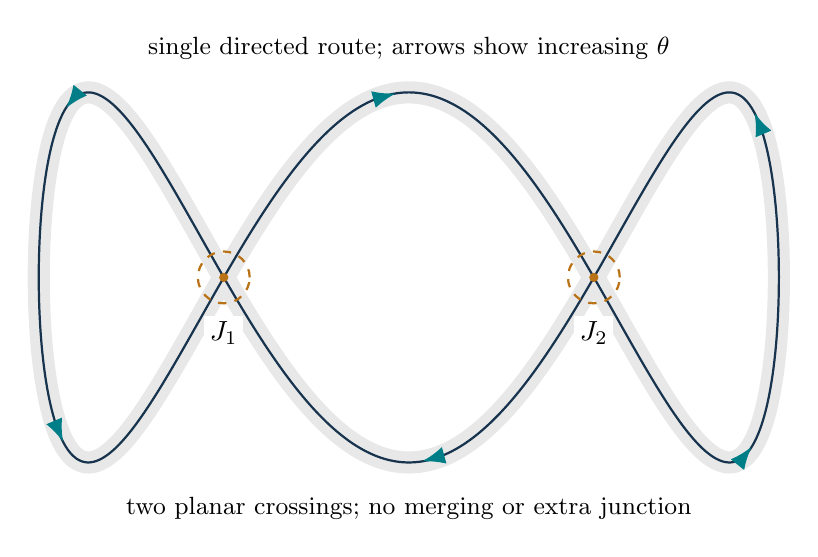
\begin{tikzpicture}[x=2.35cm,y=2.35cm,>=Latex]
 \draw[gray!18,line width=8pt,samples=501,domain=0:360,smooth,variable=\t] plot ({2*cos(\t)},{sin(3*\t)});
 \draw[navy,line width=.8pt,samples=501,domain=0:360,smooth,variable=\t] plot ({2*cos(\t)},{sin(3*\t)});
 \foreach \a in {18,85,155,198,265,335}{
  \draw[teal,very thick,->] ({2*cos(\a)},{sin(3*\a)}) -- ({2*cos(\a+3)},{sin(3*(\a+3))});}
 \foreach \x/\n in {-1/1,1/2}{
  \draw[amber,dashed,thick] (\x,0) circle (.14);
  \fill[amber] (\x,0) circle (.025);
  \node[fill=white,inner sep=2pt] at (\x,-.30) {$J_{\n}$};}
 \node[font=\small,fill=white] at (0,1.24) {\bi{single directed route; arrows show increasing $\theta$}{单条有向路线；箭头表示 $\theta$ 递增}};
 \node[font=\small,fill=white] at (0,-1.25) {\bi{two planar crossings; no merging or extra junction}{两个平面交叉点；无合流或额外路口}};
\end{tikzpicture}
\caption{\bi{Double figure-eight layout ($R/H=2$). Road width and dashed conflict regions are schematic, not to scale.}{双八字布局（$R/H=2$）。道路宽度与虚线冲突区域均为示意，不按比例绘制。}}
\end{figure}

\bi{The schematic has three enclosed lobes; it is not two independent original figure-eights joined by a merge. It expresses the agreed one-route, two-crossing topology. A physical crossing shares road space, but route branches remain fixed: vehicles cannot turn onto another branch. Build in RoadRunner as two fixed crossing junctions with branch-preserving connections and external longitudinal control.}{示意图具有三个封闭瓣区，并非通过合流连接的两个独立原八字。它实现的是已确定的“一条路线、两个交叉口”拓扑。物理路口共享道路空间，但路线分支固定，车辆不能转到其他分支。RoadRunner 中应构建两个固定交叉路口，保持分支连接，纵向控制由外部控制器负责。}

\bisubsection{Scale, curvature and event coordinates}{尺度、曲率与事件位置}
\[
 s(\theta)=\int_0^\theta\sqrt{R^2\sin^2\xi+9H^2\cos^2(3\xi)}\,d\xi,
 \qquad L=s(2\pi).
\]
\bi{For $R/H=2$ and $L=4694.8$ m, numerical integration gives $R\approx613.70$ m and $H\approx306.85$ m. The minimum centerline radius is approximately 32.31 m. At 30 km/h, the corresponding kinematic lateral acceleration is approximately 2.15 m/s$^2$; vehicle tracking must still be calibrated. The lane width is a proposed 4 m. These are new design values, not original-report parameters.}{在 $R/H=2$、$L=4694.8$ m 下，数值积分得到 $R\approx613.70$ m、$H\approx306.85$ m。中心线最小曲率半径约为 32.31 m。在 30 km/h 下，对应运动学横向加速度约为 2.15 m/s$^2$，仍需校准车辆路径跟踪。建议车道宽为 4 m。以上均为新增设计值，不是原报告配置。}

\begin{center}
\begin{tabular}{llll}
\toprule
\bi{Event}{事件} & \bi{Parameter}{参数} & \bi{Junction / branch}{路口 / 分支} & $s$ (m)\\
\midrule
$e_1$ & $\pi/3$ & $J_2/A$ & 722.67\\
$e_2$ & $2\pi/3$ & $J_1/A$ & 1624.73\\
$e_3$ & $4\pi/3$ & $J_1/B$ & 3070.07\\
$e_4$ & $5\pi/3$ & $J_2/B$ & 3972.13\\
\bottomrule
\end{tabular}
\end{center}

\begin{figure}[htbp]
\centering
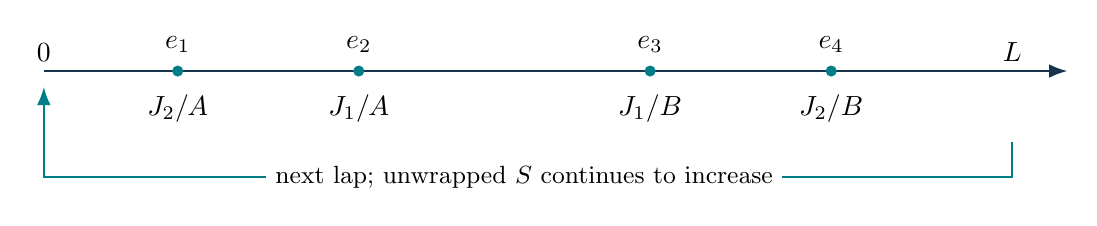
\begin{tikzpicture}[>=Latex]
 \draw[navy,thick,->] (0,0)--(13,0);
 \foreach \x/\e/\j in {1.7/1/{J_2/A},4.0/2/{J_1/A},7.7/3/{J_1/B},10.0/4/{J_2/B}}{
  \fill[teal] (\x,0) circle (2pt);
  \node[above=3pt] at (\x,0) {$e_{\e}$};
  \node[below=5pt] at (\x,0) {$\j$};}
 \node[above] at (0,0) {$0$};\node[above] at (12.3,0) {$L$};
 \draw[teal,thick,->] (12.3,-.9)--(12.3,-1.35)--(0,-1.35)--(0,-.2);
 \node[fill=white,font=\small] at (6.1,-1.35) {\bi{next lap; unwrapped $S$ continues to increase}{下一圈；展开弧长 $S$ 持续增加}};
\end{tikzpicture}
\caption{\bi{Route event order, not a physical map. Each lap has four crossing events.}{路径事件顺序，不是物理地图。每圈有四次路口通行事件。}}
\end{figure}

\bi{Consecutive event distances are approximately 902.06, 1445.34, 902.06 and 1445.34 m, including wraparound. A geometric junction separation of 613.70 m must not replace these longitudinal distances. At nominal speed, the corresponding travel times are approximately 108.25 and 173.44 s. Event order is $J_2,J_1,J_1,J_2$, not strict alternation.}{包含跨圈段在内，相邻事件的路径距离约为 902.06、1445.34、902.06 与 1445.34 m。两个路口的几何直线距离为 613.70 m，不能替代纵向路径距离。按目标速度，对应行驶时间约为 108.25 与 173.44 s。事件顺序是 $J_2,J_1,J_1,J_2$，并非严格交替。}

\bi{For every branch, obtain conflict-region entry and exit from the overlapping lane footprints, vehicle dimensions and an explicit margin. Keep these separately from the center-crossing distance used by the barrier. Do not draw a circular region and then assume it defines a validated safety threshold.}{各分支的冲突区域入口与出口，应根据车道占地重叠、车辆尺寸及明确余量确定。它们与 barrier 使用的中心交叉断面距离分别记录。不能仅画一个圆形示意区域，就将其视为经过验证的安全阈值。}

\bisection{Feedback control at two junctions}{两个路口的反馈控制}
\bisubsection{State and event interfaces}{状态与事件接口}
\bi{Use wrapped position $s_i\in[0,L)$ and unwrapped position $S_i=s_i+n_iL$. Each encounter has an event ID, junction ID, branch ID and lap index. Track route progress using the previous branch and a local projection window; nearest Euclidean point alone is ambiguous at a crossing. Center-crossing distance is the signed difference between the encounter coordinate and $S_i$.}{使用圈内位置 $s_i\in[0,L)$ 与展开位置 $S_i=s_i+n_iL$。每次路口经过均包含事件 ID、路口 ID、分支 ID 和圈数。根据上一时刻分支与局部投影窗口跟踪路径进度；仅使用最近欧氏点会在路口产生歧义。到交叉中心断面的距离为该次事件位置与 $S_i$ 的有符号差。}

\begin{tabularx}{\linewidth}{P{.23\linewidth}Y}
\toprule
\bi{Module}{模块} & \bi{Minimum interface}{最小接口}\\
\midrule
\bi{State mapping}{状态映射} & \bi{Vehicle ID, timestamp, $S_i$, $v_i$, branch/event ID, measured body dimensions.}{车辆 ID、时间戳、$S_i$、$v_i$、分支与事件 ID、实际车身尺寸。}\\
\bi{Local candidate selection}{局部候选选择} & \bi{For each junction: nearest approaching candidate per branch within $D_a$; occupied branches logged separately.}{每路口：各分支接近窗口 $D_a$ 内最近候选车；占用分支另行记录。}\\
\bi{Speed correction}{速度修正} & \bi{Two distances, gain, activation and saturation; output signed correction and activation flag.}{两个距离、增益、激活与饱和参数；输出有符号修正及激活标记。}\\
\bi{Execution and logging}{执行与记录} & \bi{Target and actual speed, throttle/brake, saturation, event crossing, rear clearance, collision and proximity records.}{目标与实际速度、油门制动、饱和、中心通行、车尾离开、碰撞及接近事件记录。}\\
\bottomrule
\end{tabularx}

\bi{The simulator may provide complete state for experiment orchestration. The barrier's decision input remains local own/conflicting-vehicle state, route geometry and a fixed branch tie rule; it does not use downstream queues or a central schedule. Ideal availability of local measurements is assumed first. This is not a demonstrated onboard perception system.}{仿真器可为实验组织提供完整状态，但 barrier 决策仅使用局部本车与冲突车状态、路线几何和固定分支平局规则，不使用下游队列或集中调度。首轮先假设局部测量理想可用；这不等同于已经实现车载感知系统。}

\bisubsection{An explicit engineering variant}{明确区分的工程改写版本}
\bi{Because original code is unavailable, label the following as a regularized distance-barrier baseline, not exact reproduction. Set $\varepsilon=0.1$ m as a numerical design default. If $|\Delta d|\ge\varepsilon$, use $\widehat{\Delta d}=\Delta d$. Otherwise set its magnitude to $\varepsilon$ with the observed sign; at exact equality, assign branch A to pass first, hence $\widehat{\Delta d}=-\varepsilon$.}{由于未获得原代码，下式应标注为“正则化距离 barrier 基线”，而非精确复现。取 $\varepsilon=0.1$ m 作为数值设计初值。当 $|\Delta d|\ge\varepsilon$ 时，取 $\widehat{\Delta d}=\Delta d$；否则将绝对值设为 $\varepsilon$，保留观测符号。严格相等时，固定 A 分支先行，因此取 $\widehat{\Delta d}=-\varepsilon$。}
\[
 u_{b,1}=\operatorname{clip}\!\left(-K_b/\widehat{\Delta d},-7,7\right),\quad
 u_{b,2}=-u_{b,1}\quad (\mathrm{km/h}).
\]
\bi{For a non-candidate or inactive pair, $u_b=0$. Compute one command per vehicle:}{非候选车辆或未激活的冲突对取 $u_b=0$。每辆车每周期生成一个指令：}
\[
 v_i^{cmd}=\operatorname{clip}\!\left(30+u_{h,i}+u_{b,i},0,40\right)\quad(\mathrm{km/h}),
 \qquad |u_{h,i}|\le10\ \mathrm{km/h}.
\]
\bi{The 40 km/h command ceiling and additive fusion are proposed choices, not confirmed original settings. Retain the report's PD/PID numbers initially, declare gap error as actual minus target spacing, and use metres/seconds for gap derivatives. Convert explicitly when entering a km/h speed loop. EMA is defined here as filtered error $\bar e_k=0.9\bar e_{k-1}+0.1e_k$; the original alpha convention is unknown.}{40 km/h 指令上限与加法融合是建议选择，不是已确认的原配置。首轮保留报告中的 PD/PID 数值，约定间距误差为实际间距减目标间距，间距导数使用 m 与 s；进入 km/h 速度环时显式换算。本文 EMA 定义为 $\bar e_k=0.9\bar e_{k-1}+0.1e_k$，原代码的 alpha 约定仍未知。}

\bi{Do not claim that a nominal barrier gain ``dominates'' headway control: saturation and opposite corrections may cancel it. Log the two components before fusion and the final clipped speed. The tie rule, reciprocal regularization and nearest-candidate reduction are heuristics, not collision-avoidance proofs. Downstream occupants remain in the occupancy ledger until their rear clears, but that ledger alone does not change the distance law or guarantee safe release.}{不能仅因增益较大，就宣称 barrier “主导”跟驰控制：饱和及相反修正仍可能抵消其作用。应记录融合前的两个分量和最终限幅速度。平局规则、倒数正则化及最近候选车筛选均为启发式处理，不是避碰证明。下游占用车辆保留至车尾离开，但占用记录本身不会改变距离控制律，也不保证安全放行。}

\bisubsection{Update order and propagation mechanism}{更新顺序与扰动传播}
\begin{figure}[htbp]
\centering
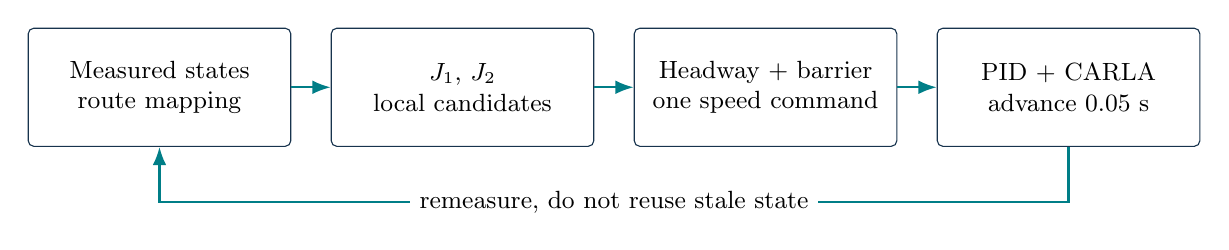
\begin{tikzpicture}[>=Latex,node distance=5mm,
 box/.style={draw=navy,rounded corners=2pt,align=center,font=\small,text width=31mm,minimum height=15mm},
 arr/.style={->,thick,teal}]
 \node[box] (state) {\bi{Measured states\\route mapping}{实际状态\\路径映射}};
 \node[box,right=of state] (local) {\bi{$J_1$, $J_2$\\local candidates}{ $J_1$、$J_2$\\局部候选车}};
 \node[box,right=of local] (speed) {\bi{Headway + barrier\\one speed command}{跟驰 + barrier\\单一速度指令}};
 \node[box,right=of speed] (plant) {\bi{PID + CARLA\\advance 0.05 s}{PID + CARLA\\推进 0.05 s}};
 \draw[arr] (state)--(local);\draw[arr] (local)--(speed);\draw[arr] (speed)--(plant);
 \draw[arr] (plant.south)--++(0,-.7)-|(state.south);
 \node[font=\small,fill=white] at ($(local.south)!0.5!(speed.south)+(0,-.7)$) {\bi{remeasure, do not reuse stale state}{重新测量，不沿用旧状态}};
\end{tikzpicture}
\caption{\bi{Synchronous state feedback; junction computations use the same snapshot.}{同步状态反馈；两个路口使用同一时刻的状态快照。}}
\end{figure}

\begin{enumerate}
\item \bi{Read one snapshot; update unwrapped progress, predecessor gaps and encounter/occupancy records.}{读取一次状态快照，更新展开位置、前车间距以及事件与占用记录。}
\item \bi{Select local candidates independently at both junctions from that snapshot.}{依据同一快照，分别选择两个路口的局部候选车。}
\item \bi{Compute headway and local barrier corrections, fuse once and execute throttle/brake commands.}{计算跟驰与局部 barrier 修正，统一融合一次后执行油门制动指令。}
\item \bi{Advance the physics by one step; detect crossing and rear-clearance transitions without resetting the same encounter prematurely.}{推进一个物理步长；检测通行与车尾离开，避免过早重置同一次路口经过事件。}
\item \bi{Record actual response and safety events, then repeat using newly measured states.}{记录实际响应及安全事件，随后使用新测量状态重复更新。}
\end{enumerate}

\bi{With 20--60 m windows, consecutive events are separated by much more than twice the window length in the proposed geometry. A vehicle therefore receives at most one local barrier correction at a time. Long-range effects arise through changed travel times and predecessor gaps, not simultaneous summation of junction commands. Any enlarged-window case that violates this separation is outside the present baseline.}{在所提几何中，20--60 m 窗口远小于相邻事件距离的一半，因此每辆车同一时刻最多接受一个局部 barrier 修正。跨路口影响通过行驶时间及前后车间距变化传播，不来自两个路口指令的同时求和。若进一步扩大窗口破坏该条件，则超出本基线适用范围。}

\bi{A correction at $J_1$ changes speed and spacing before a later $J_2$ encounter; repeated circulation returns those changes to $J_1$. Consecutive visits to the same junction also matter. Hypotheses are: compatible phases permit low-intervention circulation; incompatible phases cause recurring interventions; higher density or asymmetric path lengths amplify the coupling. All three must be tested, not asserted.}{$J_1$ 的修正改变车辆速度与间距，影响后续 $J_2$ 的到达；持续循环后，这些变化又返回 $J_1$。连续两次经过同一路口也会影响反馈。待检验假设是：相位兼容时可形成低干预循环；相位不兼容时会反复激活；更高密度或不对称路径长度可能放大耦合。这些均须实验验证。}

\Needspace{16\baselineskip}
\bisection{Configuration and matched experiments}{配置与配对实验}
\bisubsection{Parameter register}{参数登记表}
\begin{longtable}{P{.34\linewidth}P{.33\linewidth}P{.23\linewidth}}
\toprule
\bi{Parameter}{参数} & \bi{Value}{取值} & \bi{Status}{状态}\\
\midrule\endhead
\bi{Reference track length}{原轨道长度} & 2347.4 m & \bi{BSc report}{本科报告}\\
\bi{Double track length; width}{双路口长度；车道宽} & 4694.8 m; 4 m & \bi{Proposed}{建议}\\
$R/H$ & 2; \bi{diagnostics: 1.5, 3}{诊断值：1.5、3} & \bi{Proposed}{建议}\\
\bi{Target speed; timestep}{目标速度；步长} & 30 km/h; 0.05 s & \bi{BSc report}{本科报告}\\
\bi{Duration; preparation; ramp}{时长；准备；加速} & 1800 s; 5 s; 12.5 s & \bi{BSc report}{本科报告}\\
\bi{Single-junction counts}{单路口车辆数} & 51, 61, 71, 81 & \bi{BSc report}{本科报告}\\
\bi{Double-junction counts}{双路口车辆数} & 102, 122, 142, 162 & \bi{Density matched}{匹配密度}\\
\bi{Spawn noise; repetitions}{初始化扰动；重复次数} & $\pm20\%$; 30 & \bi{BSc report}{本科报告}\\
$K_b$; $D_{activation}$; $D_a$ & 25; 10 m; 20 m & \bi{Appendix B}{原附录 B}\\
\bi{Barrier correction limit}{barrier 修正上限} & $\pm7$ km/h & \bi{BSc Discussion}{原讨论章节}\\
\bi{Headway PD; EMA}{跟驰 PD；EMA} & 3.5, 1.0; 0.9 & \bi{Numbers from Appendix}{数值来自原附录}\\
\bi{Longitudinal PID}{纵向 PID} & 0.5, 0.25, 0.02 & \bi{Numbers from Appendix}{数值来自原附录}\\
\bi{Regularization; speed ceiling}{正则化；指令速度上限} & 0.1 m; 40 km/h & \bi{Engineering variant}{工程改写}\\
\bi{Command units, EMA convention}{指令单位、EMA 约定} & \bi{Explicit variant definitions}{采用改写版本的明确约定} & \bi{Original code unknown}{原代码未知}\\
\bottomrule
\end{longtable}

\bi{FAS defaults from the original Appendix B are: stop line 12 m upstream, approach window 50 m, reaction time 1 s, assumed deceleration 2.5 m/s$^2$, minimum/maximum green 12/45 s, yellow 4 s, gap-out 3.4 s, upstream detector offset 30 m, request loop length 10 m and discharge loop length 5 m. Appendix B also lists a ``maximum yellow time'' of 1 s, inconsistent with yellow 4 s. Use 4 s in the declared engineering baseline and retain the 1 s entry as an unresolved source discrepancy. Apply the same independent FAS to each junction; no green-wave offsets.}{原附录 B 中 FAS 参数为：停止线在路口上游 12 m、接近窗口 50 m、反应时间 1 s、假设减速度 2.5 m/s$^2$、最小/最大绿灯 12/45 s、黄灯 4 s、间隔终止阈值 3.4 s、上游检测器偏移 30 m、请求线圈长 10 m、放行线圈长 5 m。附录还列出“最大黄灯时间”1 s，与黄灯 4 s 不一致。声明的工程基线采用 4 s，并保留 1 s 项作为待核实的来源矛盾。两个路口分别运行同一 FAS，不加入绿波偏移。}

\bi{Freeze the installed CARLA/RoadRunner versions, map export settings, vehicle blueprints and physics parameters after a smoke test. The original report does not identify a CARLA version. Keep throttle/brake mutually exclusive and avoid velocity overrides after initialization. Record simulator collision protection, intervention, removal and respawn behavior rather than attributing it to the controller.}{在试运行后冻结实际安装的 CARLA/RoadRunner 版本、地图导出设置、车辆蓝图和物理参数。原报告未明确 CARLA 版本。油门与制动互斥，初始化后不直接覆盖车辆速度。记录仿真器的碰撞保护、干预、移除及重新生成行为，不能将这些机制计入控制器自身能力。}

\bisubsection{Experiment stages and controls}{实验阶段与对照}
\begin{enumerate}
\item \bi{Reference check: rebuild the original single-junction geometry and run the regularized barrier and FAS at the four original counts. Compare qualitative trajectories; exact numeric reproduction remains unclaimed without original code.}{参考检查：重建原单路口几何，在四组原车辆数下运行正则化 barrier 与 FAS。比较定性轨迹；缺少原代码时不宣称精确数值复现。}
\item \bi{Primary double-junction experiment: compare regularized barrier and independent FAS at the four doubled counts. Use 30 paired seeds (0--29), with identical spawn/type assignments within each comparison. Use separate tuning seeds 100--109.}{双路口主实验：在四组翻倍车辆数下，对比正则化 barrier 与独立 FAS。采用 30 个配对种子（0--29），每组控制器共享初始化与车型分配。调参种子另用 100--109。}
\item \bi{Geometry diagnostic: hold $L$, density and controller fixed; vary $R/H$ over 1.5, 2, 3. At 1.5 the minimum radius is about 20.21 m, so tracking and lateral acceleration are a confound. Calibrate before use; if the common speed is infeasible, classify it as a geometry stress case, not a clean coupling comparison.}{几何诊断：固定 $L$、密度和控制器，比较 $R/H=1.5,2,3$。比例 1.5 时最小半径约为 20.21 m，跟踪能力与横向加速度会成为混杂因素。先校准；若共同速度不可行，则归为几何压力案例，而非纯耦合对比。}
\item \bi{Control-window diagnostic: vary $D_a=20,40,60$ m at fixed geometry and density, leaving gain and activation distance unchanged. Repeat at $N-1$ and $N+1$ to examine initialization phase/parity, separately from the matched-density main experiment.}{控制窗口诊断：固定几何和密度，比较 $D_a=20,40,60$ m，保持增益与激活距离不变。另在 $N-1$ 与 $N+1$ 下检查初始化相位与奇偶性，独立于匹配密度的主实验。}
\end{enumerate}

\bi{At doubled $L$ and $N$, target center spacing $L/N$ remains the original value. Even counts use equal type numbers. Odd diagnostics use one extra Tesla. Treat spacing as center-to-center unless explicitly converting to bumper gap. Use safe spawn screening outside both conflict regions with full vehicle footprints; do not snap several vehicles to the same safe waypoint. Reject and resample an entire infeasible placement with deterministic attempt indexing, recording every rejection.}{长度与车辆数同时翻倍后，目标中心间距 $L/N$ 与原报告一致。偶数车辆使用相同数量的两种车型；奇数诊断中 Tesla 多一辆。间距默认指中心到中心距离，若转换为车身净间距必须明确。初始化时按完整车身占地排除两个冲突区域，避免将多辆车吸附到同一安全路点。对于不可行的整组位置，按确定性的尝试索引重新采样，并记录所有拒绝。}

\bi{Primary runs last 1800 s. Report initialization/ramp separately, the early transient through 600 s, and the later 600--1800 s window, without automatically calling it steady state. A declared non-convergence follow-up may extend every seed of an affected condition to 3600 s; do not extend only favorable runs.}{主实验时长为 1800 s。分别报告初始化与加速阶段、截至 600 s 的早期瞬态，以及 600--1800 s 的后期窗口，不自动将后期称为稳态。若某条件未收敛，可按事先声明的后续实验将该条件的全部种子延长至 3600 s，不能只延长有利样本。}

\bisection{Metrics, analysis and acceptance tests}{指标、分析与验收测试}
\bisubsection{Comparable network accounting}{可比较的网络统计口径}
\bi{Count passage once per vehicle/event/lap using a signed-distance transition, rather than counting frames spent near a crossing. Report each $Q_j=C_j/T$ separately, plus route lap completions $Q_{lap}$. A lap has two crossing events in the original geometry and four in the new one. Consequently the sum $Q_1+Q_2$ cannot alone demonstrate a throughput improvement over the single intersection. At uniform target speed the kinematic references are $Q_{lap}=Nv^*/L$ and total crossing rate $4Nv^*/L$ for the new path. They are nominal-speed references, not strict upper bounds when commanded speeds exceed $v^*$.}{按车辆、事件和圈数，以有符号距离跨越计数，每次通行只计一次，不能将停留在路口附近的每帧都算作通行。分别报告 $Q_j=C_j/T$ 及整圈完成率 $Q_{lap}$。原路线每圈两次通行，新路线每圈四次，因此仅凭 $Q_1+Q_2$ 不能认定相对单路口的吞吐量提升。匀速目标速度下，新路线的运动学参考值为 $Q_{lap}=Nv^*/L$ 与总通行率 $4Nv^*/L$。若指令速度允许超过 $v^*$，这些是目标速度参考值，不是严格上界。}

\bi{Delay is actual completed-lap time minus a one-vehicle free-flow lap time on the same geometry and tracking setup. Also report incomplete laps and elapsed time; clipping negative delay to zero must not be silently introduced. Energy is total battery kWh divided by actual traveled kilometres, with type-stratified results. Report collision contacts, overlapping occupancy of conflicting branches and the original-style 5 m proximity threshold separately. Because the source does not define its exact proximity implementation, use a declared new criterion: at one candidate's center crossing, count an event if the opposite approaching candidate is less than 5 m from its center crossing, deduplicated by vehicle pair and encounter. This is a proximity event, not a reproduced original collision count.}{延误为完成一圈的实际时间减去同几何、同跟踪设置下单车自由流圈时。另报告未完成圈次及已行驶时间，不能静默将负延误截断为零。能耗为总电池 kWh 除以实际行驶 km，并按车型分层。几何接触、冲突分支区域占用重叠及原风格的 5 m 接近阈值分别统计。原文未定义接近事件的准确实现，因此声明一个新判据：某候选车中心过线时，若另一冲突分支接近车到其中心断面不足 5 m，则记录一次；按车辆对与事件去重。这是接近事件，不是已复现的原碰撞计数。}

\bi{Track activation frequency, headway RMS error, minimum body clearance, speed/acceleration variability, command saturation and stops (speed below 0.1 m/s for at least 1 s). Operational convergence means all center-spacing errors stay within 2.5 m and no barrier activation occurs for at least one nominal full-lap duration. This is a measured criterion, not stability proof. Use cross-correlation or event-aligned changes in speed/gap between junctions to estimate propagation delay; distinguish association from causality.}{记录激活频率、车间距 RMS 误差、最小车身间距、速度与加速度波动、指令饱和及停车（速度低于 0.1 m/s 持续至少 1 s）。操作性收敛定义为：全部中心间距误差保持在 2.5 m 内，且至少一个目标速度完整圈时内无 barrier 激活。这是测量判据，不是稳定性证明。通过两路口速度或间距变化的互相关及事件对齐估计传播时延，并区分统计关联与因果结论。}

\bi{Compute metrics per seed first. Report means and paired method differences with seed-level bootstrap 95\% intervals (10,000 resamples, fixed analysis seed 20261007). Do not treat vehicle observations as independent experimental repetitions. Preserve all failed runs, controller interventions and uncompleted trajectories.}{先按种子计算指标，再报告均值与方法间配对差，采用种子层面的 bootstrap 95\% 区间（10,000 次重采样，分析种子固定为 20261007）。不能将同次运行内的车辆观察视为独立实验重复。保留所有运行失败、控制干预及未完成轨迹。}

\bisubsection{Required scenarios before batch experiments}{批量实验前的必查场景}
\begin{tabularx}{\linewidth}{P{.35\linewidth}Y}
\toprule
\bi{Scenario}{场景} & \bi{Acceptance observation}{验收观察}\\
\midrule
\bi{One vehicle, multiple laps}{单车连续绕圈} & \bi{Exactly four events per lap; no false pairs or progress jumps.}{每圈恰好四次事件，无虚假冲突对或路径位置跳变。}\\
\bi{Equal distance; unequal speeds}{等距离；不同速度} & \bi{Finite deterministic commands; differing behavior is logged, not declared safe.}{指令有限且确定；记录行为差异，不预先认定安全。}\\
\bi{Crossing and lap boundary}{过路口与跨圈} & \bi{Correct branch IDs, one crossing count and rear-clearance retention.}{分支 ID 正确、通行只计一次、车尾未离开时保留占用。}\\
\bi{Two followers and a crossing car}{两辆跟驰车与横向来车} & \bi{Headway/barrier cancellation, saturation and collisions remain visible.}{跟驰与 barrier 抵消、饱和及碰撞均可观察。}\\
\bi{Dense randomized initialization}{高密度随机初始化} & \bi{Safe spawning; transient violations and rejected placements reported.}{生成时无车身重叠；报告瞬态违规及位置拒绝。}\\
\bi{One-junction speed perturbation}{单路口速度扰动} & \bi{Follow perturbation through downstream visits and back around the loop.}{追踪扰动经过下游路口并绕回的过程。}\\
\bi{0.05 s versus 0.025 s replay}{0.05 s 与 0.025 s 重放} & \bi{Check sampling sensitivity and independent body/occupancy events.}{检查采样敏感性及独立车身和占用事件。}\\
\bottomrule
\end{tabularx}

\clearpage
\bisection{Implementation roadmap and decision boundary}{实施路线与决策边界}
\begin{enumerate}
\item \bi{Geometry milestone: generate the curve and arc-length table, verify exactly two crossings, four encounters, curvature and branch connections; calibrate one vehicle.}{几何阶段：生成曲线与弧长表，验证两个交叉点、四次经过、曲率及分支连接；完成单车校准。}
\item \bi{Control milestone: implement the declared regularized baseline and independent FAS, verify state/event bookkeeping, then test transient failure cases.}{控制阶段：实施声明的正则化基线与独立 FAS，验证状态和事件记录，再检查瞬态失败案例。}
\item \bi{Experiment milestone: freeze configuration and tuning, execute paired seeds, analyze efficiency together with safety and convergence.}{实验阶段：冻结配置及调参结果，运行配对种子，将效率、安全和收敛一并分析。}
\item \bi{Extension milestone: only after diagnosing the coupling, consider local adaptive gain or occupancy-aware release as separately named variants. Shared-state junction coordination and acceleration-QP filtering remain outside the present method.}{拓展阶段：诊断耦合机制后，再将局部自适应增益或占用感知放行作为独立命名的改进版本。共享状态路口协调与加速度 QP 过滤不属于当前方法。}
\end{enumerate}

\bi{A useful study may discover a failure boundary rather than improved performance. The main deliverable is an auditable relationship between geometry, density, local interventions and global circulation. If repeated interventions persist or transient safety worsens, report those outcomes and narrow the operating domain before adding more junctions.}{研究可能发现的是失效边界，而非性能提升。核心交付是可核查的几何、密度、局部干预与全局循环之间的关系。若持续反复激活或瞬态安全恶化，应如实报告，并先收缩适用范围，再增加路口数量。}

\bisection{Appendix: files, pseudocode and open items}{附录：文件、伪代码与待核实事项}
\begingroup\small
\bi{The editable package includes the main file (main.tex), bilingual body (report\_body.tex), bibliography (references.bib), design register (proposed\_config.json), geometry results (geometry\_summary.json), and checker (geometry\_check.py). The body is rendered twice with one language switch, sharing formulas and TikZ geometry. Build with \texttt{latexmk -xelatex main.tex}.}{文件包包括主文件（main.tex）、双语正文（report\_body.tex）、文献库（references.bib）、设计登记表（proposed\_config.json）、几何结果（geometry\_summary.json）与检查脚本（geometry\_check.py）。正文通过语言开关渲染两次，共用公式与 TikZ 几何。使用 \texttt{latexmk -xelatex main.tex} 编译。}

\begin{quote}\small
\bi{Initialize map, vehicles, event ledger and logs. For each synchronous tick: snapshot state; map route progress; update predecessor and occupancy records; select the two local pairs; calculate PD and active regularized corrections; fuse/clamp the speed once; execute PID throttle/brake; advance CARLA; record actual response and events. After each run: preserve failures and unfinished laps; aggregate per seed.}{初始化地图、车辆、事件台账与日志。每个同步周期：获取状态快照；映射路径进度；更新前车与占用记录；选择两个局部冲突对；计算 PD 和激活的正则化修正；统一融合并限幅速度；执行 PID 油门制动；推进 CARLA；记录实际响应和事件。每次运行结束：保留失败与未完成圈次，按种子汇总指标。}
\end{quote}

\bi{Open items before executable experiments: original controller code and signal phase details; speed-loop units and PID discretization; EMA convention; handling of rear occupancy; original proximity counter; map export/version compatibility; blueprint dimensions and per-type braking/tracking calibration. No executable API is added to the project by this document. The JSON is a design register, not a working CARLA configuration.}{运行仿真实验前，仍需核实原控制代码与信号相位细节、速度环单位及 PID 离散化、EMA 约定、车尾占用处理、原接近事件计数器、地图导出与版本兼容、车辆蓝图尺寸，以及各车型的制动和跟踪表现。本文件不新增可执行控制 API；JSON 用于登记设计参数，不能直接作为 CARLA 配置运行。}
\endgroup

\clearpage
\nocite{carla}
\renewcommand{\refname}{References / 参考文献}
\addcontentsline{toc}{section}{References / 参考文献}
\bibliographystyle{unsrt}
\bibliography{references}
\end{document}
